\documentclass[hyperref,UTF-8]{ctexart}

\usepackage[strict]{changepage}
\usepackage{graphicx}?
\usepackage{float}

\usepackage{fancyhdr}

% ------------------------ 数学公式必备 ------------------------
\usepackage{amsmath}
\usepackage{newtxtext}
\usepackage{amssymb}
\usepackage{mathrsfs}
\usepackage{bm}

% ------------------------ 页边距排版 ------------------------
\usepackage{geometry}
\geometry{a4paper,left = 2.5cm, right = 2.5cm, top = 2.5cm, bottom = 2.5cm}


% ------------------------ 自定义颜色 ------------------------
\usepackage[dvipsnames,svgnames]{xcolor}
\usepackage{tcolorbox}
\tcbuselibrary{most}
\definecolor{examplecolor}{rgb}{0.77,0.72,0.65} % 莫兰迪棕色
\definecolor{blueshade}{rgb}{0.95,0.95,1} % 蓝色文本框,竖线颜色设为 RoyalBlue
\definecolor{greenshade}{rgb}{0.90,0.99,0.91} % 绿色文本框,竖线颜色设为 Green
\definecolor{redshade}{rgb}{1.00,0.90,0.90}% 红色文本框,竖线颜色设为 LightCoral
\definecolor{brownshade}{rgb}{0.99,0.97,0.93} % 棕色文本框,竖线颜色设为 BurlyWood


% ------------------------ 文本框 ------------------------
\usepackage{framed}


% 橙色文本框 
\newtcolorbox{justification}[2][]
{enhanced,breakable,
left=12pt,right=12pt,% 左右边距
% fonttitle=\bfseries, % 可以设置标题是否粗体
coltitle=white, % 标题字体颜色
colbacktitle=BurntOrange, % 标题背景颜色
attach boxed title to top left={yshifttext=-1mm},
boxed title style={skin=enhancedfirst jigsaw,arc=1mm,bottom=0mm,boxrule=0mm},
boxrule=1pt, % 边框线宽
%
colback=white, % 文本框背景颜色
colframe=BurntOrange, % 框线颜色
%
sharp corners=northwest,
% drop fuzzy shadow, % 可以选择是否设置阴影效果
title=\vspace{3mm}#2,
arc=1mm,
#1}%


% 蓝色文本框
\newtcolorbox{understanding}[2][]
{enhanced,breakable,
left=12pt,right=12pt,% 左右边距
% fonttitle=\bfseries, % 可以设置标题是否粗体
coltitle=white, % 标题字体颜色
colbacktitle=RoyalBlue, % 标题背景颜色
attach boxed title to top left={yshifttext=-1mm},
boxed title style={skin=enhancedfirst jigsaw,arc=1mm,bottom=0mm,boxrule=0mm},
boxrule=1pt, % 边框线宽
%
colback=white, % 文本框背景颜色
colframe=RoyalBlue, % 框线颜色
%
sharp corners=northwest,
% drop fuzzy shadow, % 可以选择是否设置阴影效果
title=\vspace{3mm}#2,
arc=1mm,
#1}%


% ------------------- 参考文献使用 BibTeX + natbib 宏包 -------------------
% 顺序编码制
% \usepackage[sort]{natbib}
% \bibliographystyle{ustcthesis-numerical}
\usepackage{cite}
\bibliographystyle{plain}


% ------------------------ 超链接 ------------------------
\usepackage[colorlinks,linkcolor = Black]{hyperref}
\hypersetup{
colorlinks = true,
linkcolor = Black,
filecolor = Black,
bookmarks = true,
urlcolor = RoyalBlue,
citecolor = cyan,
bookmarksopen = false,
pdfpagemode = FullScreen,
pdfstartview = Fit
}

% ------------------------ 自定义命令 ------------------------
\newcommand{\R}{\mathbb{R}}
\newcommand{\F}{\mathbb{F}}
\newcommand{\N}{\mathbb{N}}
\newcommand{\Q}{\mathbb{Q}}
\newcommand{\Z}{\mathbb{Z}}
\newcommand{\E}{\text{E}}
\newcommand{\Cov}{\text{Cov}}
\newcommand{\Var}{\text{Var}}
\newcommand{\0}{\boldsymbol{0}}
\newcommand{\setparDis}{\setlength{\parskip} {0.3cm} }

% ------------------------ 其他设置 ------------------------
\CTEXsetup[format={\bfseries}]{section}
\CTEXsetup[format={\bfseries}]{subsection}

\linespread{1.55}

\newcommand{\enabstractname}{Abstract}
\newcommand{\cnabstractname}{摘要}
\newenvironment{enabstract}{%
  \par\small
  \noindent\mbox{}\hfill{\bfseries \enabstractname}\hfill\mbox{}\par
  \vskip 2.5ex}{\par\vskip 2.5ex}
\newenvironment{cnabstract}{%
  \par\small
  \noindent\mbox{}\hfill{\bfseries \cnabstractname}\hfill\mbox{}\par
  \vskip 2.5ex}{\par\vskip 2.5ex}


\begin{document}
\setparDis
\nocite{*}

\begin{center}
    \heiti \fontsize{24pt}{0}{泊松流生成模型}

    \vspace{12pt}

    \kaishu \fontsize{13.75pt}{0}译者:任宇轩、禤科材\footnotetext{\textbf{论文原文:}\href{https://arxiv.org/abs/2209.11178}{Poisson Flow Generative Models}}
\end{center}

\begin{cnabstract}
    我们提出了一种新的“泊松流”生成模型(PFGM),它将高维半球上的均匀分布转化为任何数据分布。 我们将数据点解释为空间中 $z = 0$ 超平面上的电荷,但增加了一个额外的维度 $z$,并由此产生高维电场(泊松方程解的梯度)。 我们证明在这些电荷沿着电场线上流动的过程中,它们在 $z = 0$ 平面上的初始分布将会变换为半径为 $r$ 的半球上的分布,并且这一分布在 $r \rightarrow \infty$ 极限内变得均匀。 为了学习这个双射变换,我们选择估计在这一增广空间中的归一化泊松场。抽样方面,本文设计了一个后向常微分方程,该常微分方程由物理上有意义的附加值锚定维度:$z$ 达到 $0$ 的同时,认为样本到达未增强数据所处的流形。 实验中,PFGM 是当前在 CIFAR-10 数据集上具有最优良性能的归一化流模型,其初始分数为 $9.68$,FID 分数为 $2.35$。 它还具有与最先进的 SDE 方法相当的性能。与此同时它还为图像生成任务提供 $10$ 倍到 $20$ 倍的加速。 此外,PFGM 在较弱的网络架构上似乎更能容忍估计错误并且对欧拉方法中的步长误差具有鲁棒性。论文代码可以在 \href{https://github.com/Newbeeer/poisson_flow}{这里} 找到。
\end{cnabstract}

\section{简介}

深度生成模型是一种重要的数据生成方法,目前已被用于生成图像、文本和音频的高质量样本,并且在改进半监督学习、领域泛化和模仿学习中也有一定应用。 然而,当前的深度生成模型也存在局限性,例如训练目标不稳定(GAN )和样本质量低(VAE,归一化流)等问题。 为此也涌现出一些新技术来稳定基于 CNN 或基于 ViT 的 GAN 模型的训练。尽管最新进展表明,扩散模型(diffusion)和基于评分的模型(scored-based models)在没有对抗性训练的情况下实现了与 GAN 相当的样本质量,但这些模型的随机采样过程很慢。 而另一篇文章提出向后 ODE 采样器(归一化流)来加速采样过程,但这些方法尚未与 SDE 的对应方法相媲美。

在此,我们利用了一个可推广到 $N$ 维的显着物理事实,提出了一种全新的泊松流生成模型(PFGM)。 即如图 1(a)所示,粘性流体中的运动将任何平面电荷分布转变为均匀的角分布。 具体来说,我们将 $N$ 维数据点 $x$(例如图像)解释为充满粘性液体(例如蜂蜜)的 $N + 1$ 维空间(见图 1(a))的 $z = 0$ 平面中的正电荷,那么 $z > 0$ 的正电荷将被其他电荷排斥并沿其排斥力的方向移动,最终穿过半径为 $r$ 的假想半球。 值得注意的是,如果原始电荷分布在 $z = 0$ 上方释放,则该运动定律将导致它们与半球的交叉点在 $r → ∞$ 极限下呈均匀分布。

我们泊松流模型的生成过程则是反转了上述的正向过程:首先在半球上生成均匀分布的负电荷,然后将它们的运动跟踪回 $z = 0$ 平面,在那里它们将作为新的数据分布。 泊松流可以被视为一种连续归一化流,因为它是一个任意分布和一个易于采样的分布之间连续映射:在之前的工作中使用的是 $N$ 维高斯分布,而在 PFGM 中是 $N$ 维半球上的均匀分布。在实践中,我们通过求解一对由电场引起的前向/后向常微分方程(ODE)(图 1(b))来实现泊松流,该方程实际上是库仑定律的 $N$ 维版本( 以数据为源的泊松方程的解)。 我们将这个高维函数的梯度相应地称为泊松场,因为“电场:一词通常指的是 $N = 3$ 的特殊情况。

\begin{figure}[ht]
  \centering
  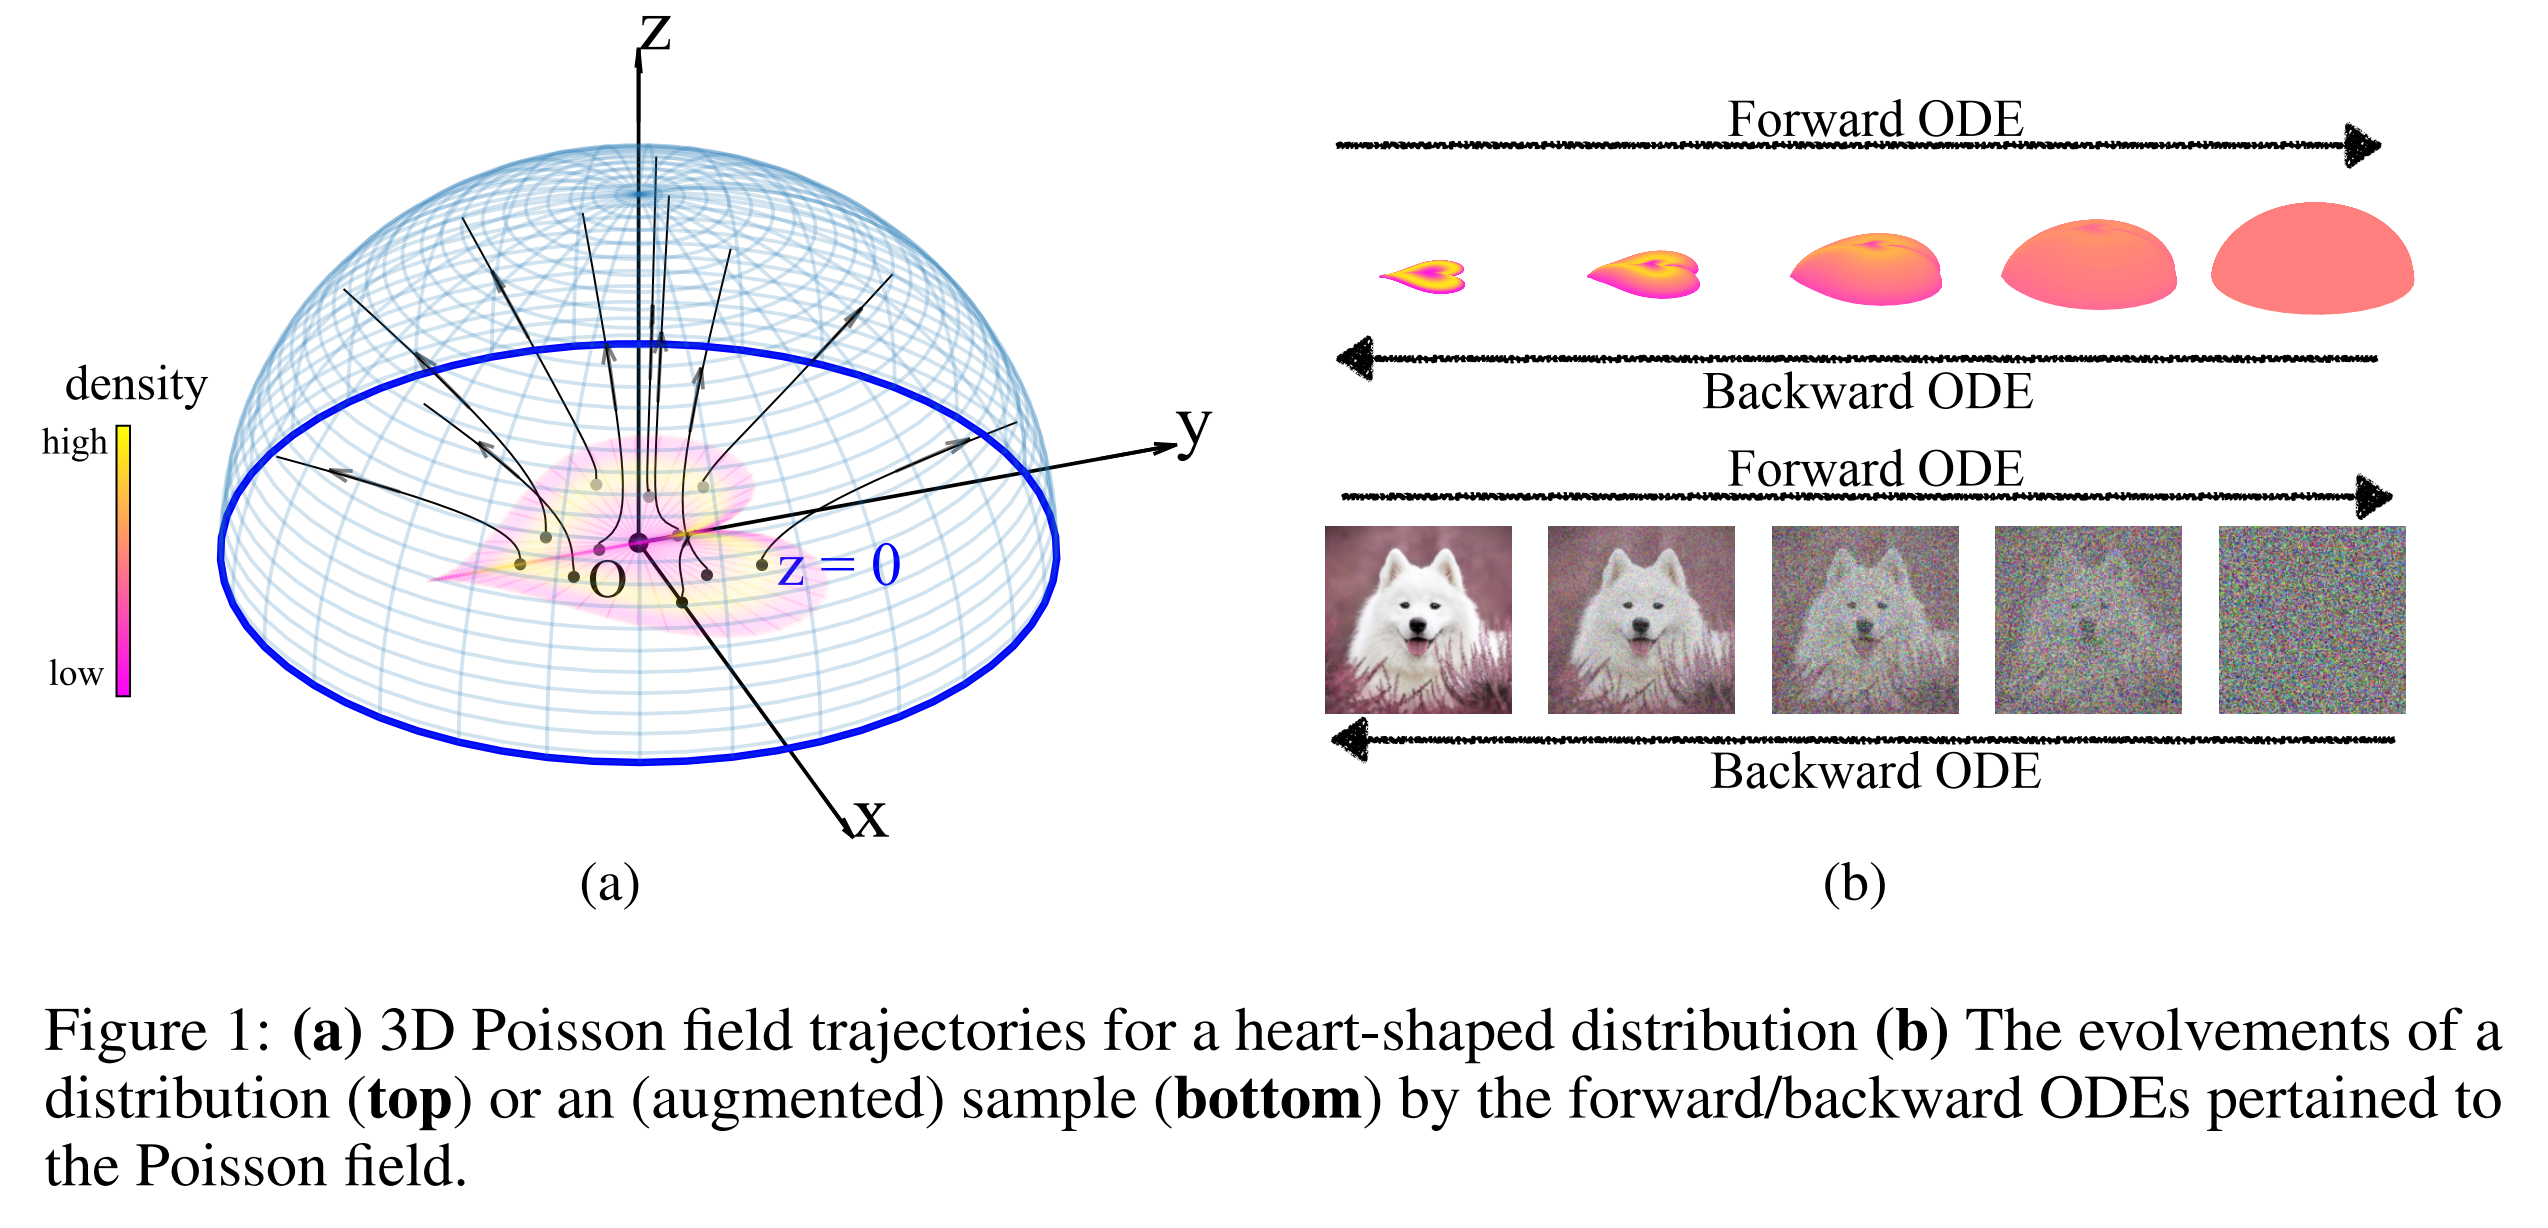
\includegraphics[width=1\textwidth]{img/figure1.png}
\end{figure}

我们提出的生成模型 PFGM 具有稳定的训练目标,并且在实验上优于以前最先进的连续流方法。 作为一种不同的迭代方法,与基于评分的方法相比,PFGM 具有两个优点。 首先,PFGMva 的 ODE 过程比文献[33]中的 SDE 采样器实现了更快的采样速度的同时保持了相近的性能;其次,我们的后向 ODE 表现出比 VE/VP/sub-VP SDE [33] 的反向 ODE 更好的生成性能,并且在较弱的架构 NSCNv2 上具有更高的稳定性。这一稳健性的基本原理如下:对于 NSCNv2,这些 ODE 基线中的时间变量与训练期间的样本范数密切相关,所以导致推断的容错性较差;相比之下,PFGM 中锚定变量与样本范数之间的联系弱得多。

在实验中,我们发现 PFGM 在归一化流系列中的 CIFAR-10 数据集上实现了当前最优良的性能,FID/Inception 分数为 2:48/9:65(w/ DDPM++ [33]) 和 2 :35/9:68(w/ DDPM++ deep [33])。 它的性能相较于当前最先进的 SDE 采样器 [33] 非常有竞争力,并且在多个数据集上实现了 10 到 20 倍的速度提升。 值得注意的是,PFGM 中的后向 ODE 是唯一一个基于 ODE 的采样器,可以在 NCSNv2 [32] 上自行生成较好的样本,而其他 ODE 在基线没有更正的情况下就会出错。 此外,PFGM 还具有对欧拉方法中步长的鲁棒性。我们进一步展示了泊松场的可逆前向/后向 ODE 在似然评估和图像处理方面的实用性,以及它在 LSUN $256 \times 256$ 数据集上对更高分辨率图像的可扩展性。

\section{背景与相关工作}

\textbf{泊松方程}\quad 在物理学中,泊松方程是一个偏微分方程,它描述了电荷分布在电场中的作用。 在 $N$ 维空间中,泊松方程可以写成:
\begin{equation}
    \nabla^2 \varphi(x) = -\rho (x)
\end{equation}
其中 $\varphi(x)$ 称为势函数,$\nabla^2  =\displaystyle \sum _{i=1}^N \frac{\partial ^2 }{\partial x_i ^2}$ 是拉普拉斯算子。我们通常定义势函数的梯度 $E(x) = -\nabla \varphi(x)$,并将泊松方程写为 $\nabla \cdot E(x) = \rho(x)$ ,这在物理学上称为高斯定律。泊松方程在物理学中应用广泛,如果将 $\rho(x)$ 解释为质量密度或电荷密度,则分别产生了牛顿引力理论 [9] 和静电理论 [11]。 $E$ 是电场的 $N$ 维模拟。 泊松方程 (1)(无穷远为零边界条件)存在唯一的简单积分解
\begin{equation}
    \varphi(x) = \int G(x,y)\rho(y) dy,\quad G(x,y) = \frac{1}{(N-2)S_{N-1}(1)} \frac{1}{|x-y|^{N-2}}
\end{equation}
其中 $S_{N-1}(1)$ 是 $(N - 1)$ 维单位球体表面积的几何常数,$G(x,y)$ 是格林函数在 $N$ 维空间中的扩推广. 函数 $\varphi(x)$ 的负梯度场则称为源 $\rho$ 的泊松场,为
\begin{equation}
    E(x) = -\nabla \varphi(x) = -\int \nabla_x G(x,y)\rho(y) dy = \int \frac{x-y}{|x-y|^N} \rho(y) dy
\end{equation}
定性来看,泊松场 $E(x)$ 远离源,或者等效地 $-E(x)$ 指向源,如图 1 所示。很容易看到,当 $ρ(x) → \delta(x - y)$ 时 ,我们得到 $E(x) \rightarrow -\nabla_x G(x,y)$ 和 $E(x) \rightarrow -\nabla_x G(x,y)$。 这意味着 $G(x,y)$ 和 $-\nabla_xG(x,y)$ 可以解释为由单位点源(例如位于 $y$ 的点电荷)生成的势函数和梯度场。 当 $\rho(x)$ 采用一般形式但有界时,显然存在渐进关系 $\|x\|\gg  \| y\|$ 。 对于最低阶,$E(x) = \nabla_xG(x;y)|_{y=0} \backsim x/\|x\|^N$ 表现为就像它是由 $y = 0$ 处的单位点源生成的一般。在物理学中,幂律衰减被认为是长程的(与指数衰减相比)[11]。

\textbf{泊松场中的粒子动力学}\quad 泊松场定义了一个流模型,其中概率分布按照梯度流$\displaystyle \frac{\partial p_t(x)}{\partial t} = -\nabla \cdot[p_t(x)E(x)]$演化。 梯度流是福克-普朗克方程[28]的特例,其中扩散系数为零。 直观上,我们其实可以将 $p_t(x)$ 视为一群粒子。 相应的 Ito 过程(非扩散)情况是前向 ODE: $\displaystyle \frac{d x}{dt} = E(x)$。 我们可以将 ODE 的轨迹解释为根据泊松场 $E(x)$ 移动的粒子,而其初始状态取自概率密度 $p_0$。 这一正向常微分方程的物理图像是在过阻尼极限下的电场中的带电粒子的运动(详细信息参见附录 F)。

\textbf{通过 ODE 进行生成建模}\quad 通过 ODE 定义的映射可以将均匀分布转换为任意数据分布来完成生成建模。 基于 ODE 的采样器允许自适应采样、精确似然估计和连续时间动态建模 [4, 33]。 此前的工作大致分为两类。 [4, 3] 引入了一种连续时间归一化流模型,该模型可以通过变量瞬时变化公式 [4] 进行最大似然训练。 为了进行采样,他们直接将学习到的可逆映射对时间进行积分。 另一项工作[33]将基于评分的模型[31, 32]和扩散模型[16]统一为一般的扩散过程,并使用扩散过程的逆时 ODE 进行采样。 他们指出,逆时常微分方程可以通过改进的架构产生高质量的样本。

\section{泊松流生成模型}

在本节中,我们从增广空间中泊松流的性质开始,展示如何通过遵循泊松的向后 ODE 从数据分布中抽取样本
的流程(第 3.1 节)。然后我们将讨论如何从数据中实际学习归一化泊松场,并通过模拟前向 ODE( 3.2 节)进行采样,并给出等效的 z 指数衰减的后向 ODE(第 3.3 节)。

\begin{figure}[ht]
  \centering
  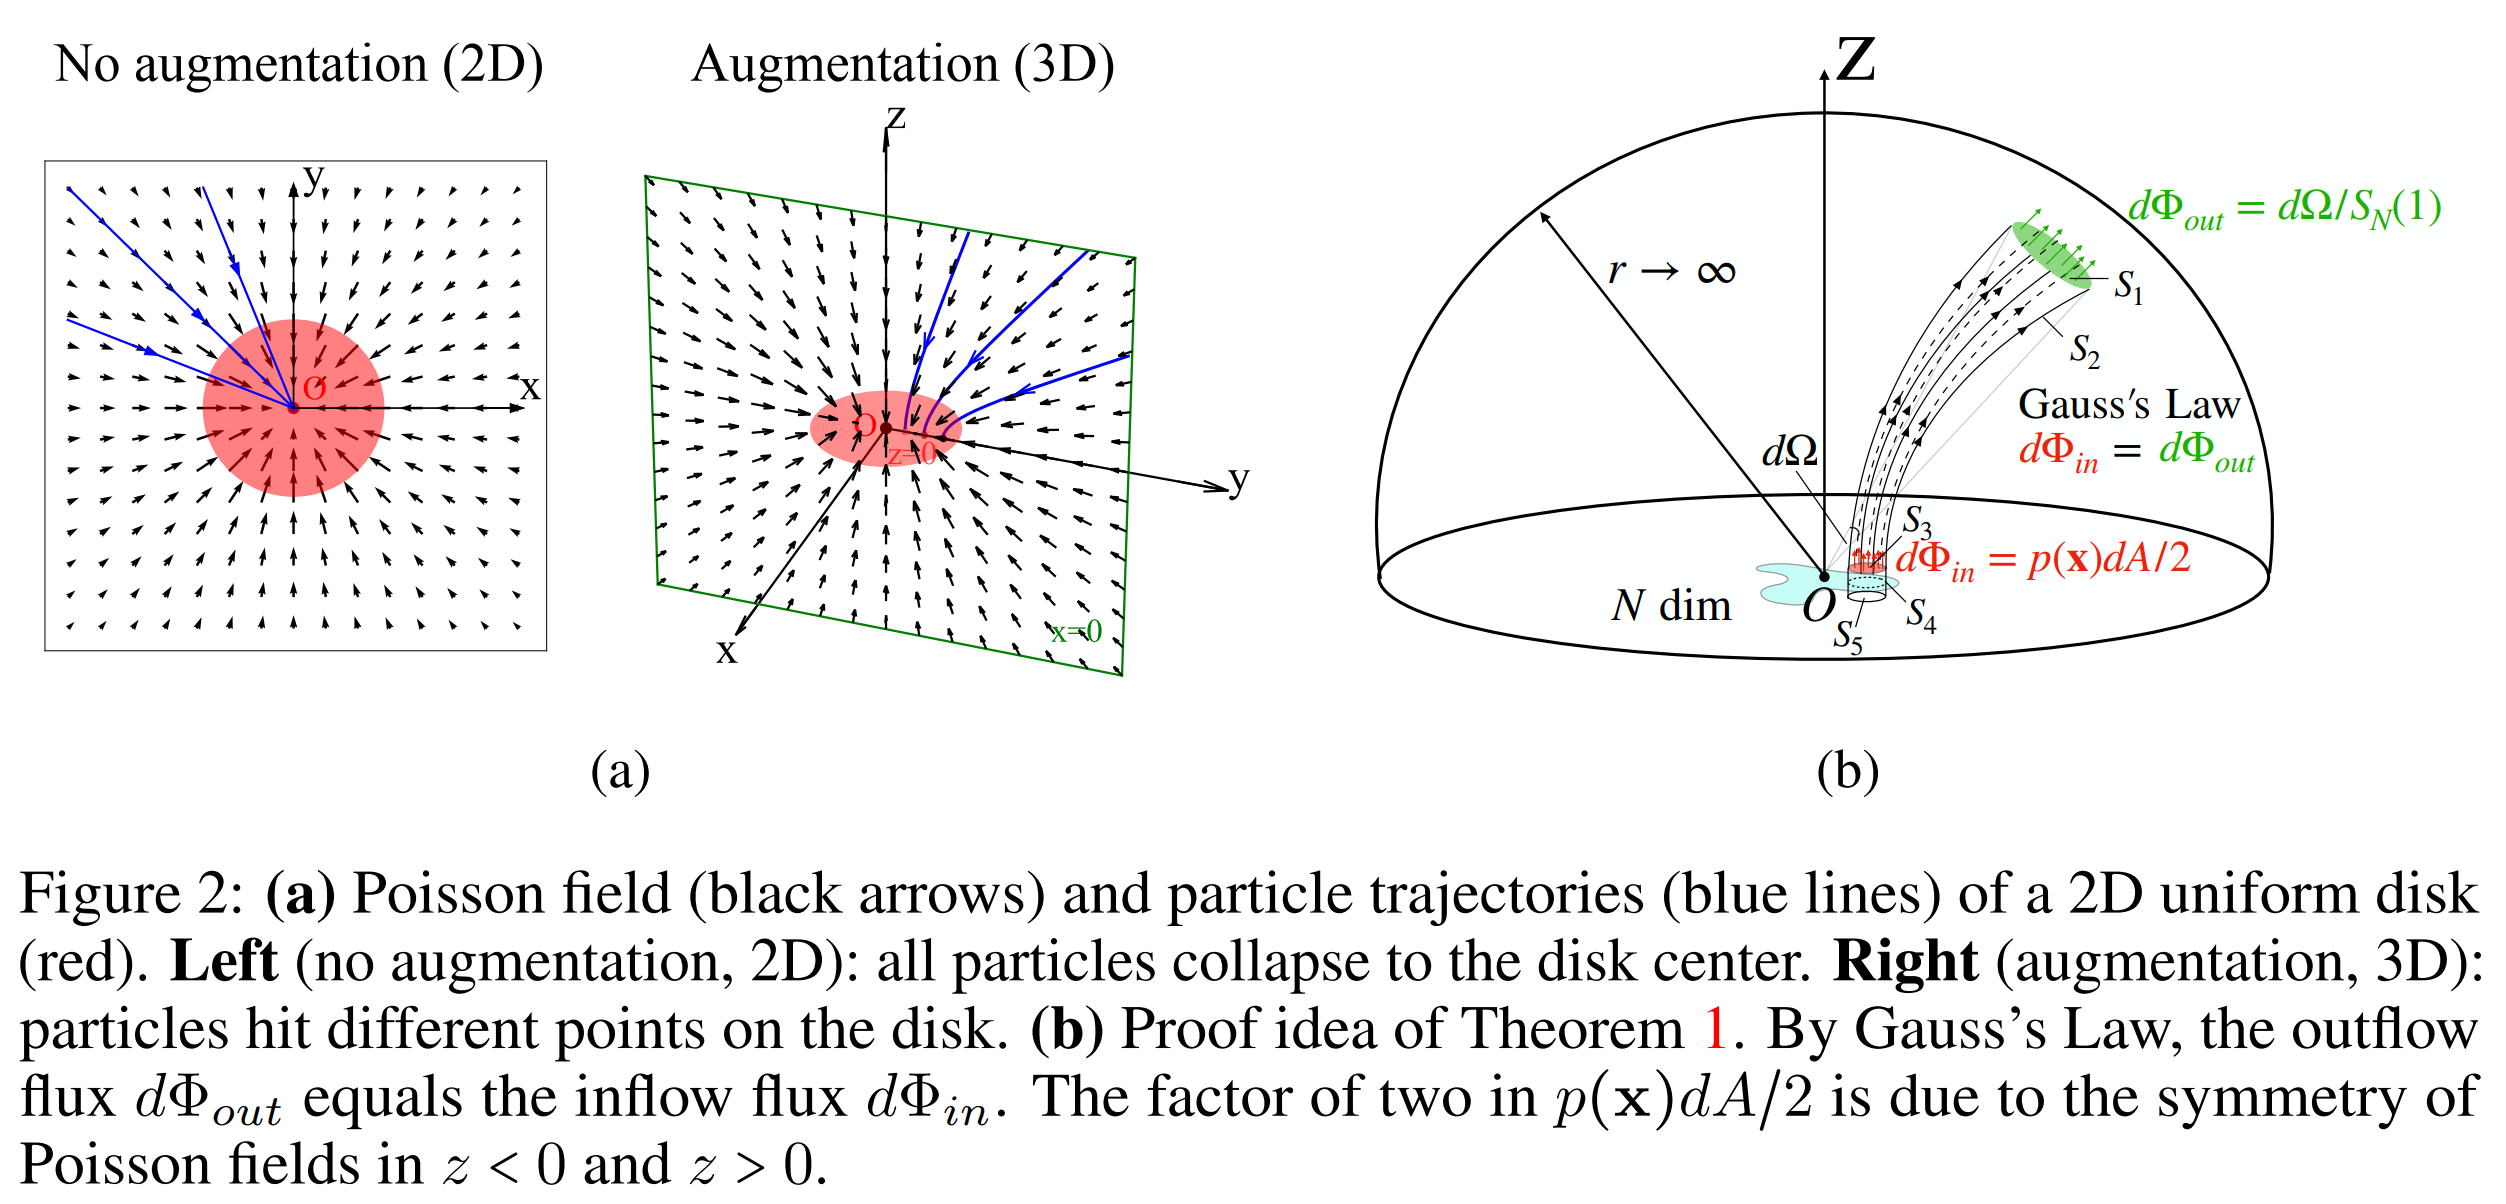
\includegraphics[width=1\textwidth]{img/figure2.png}
\end{figure}

\subsection{使用附加维度增强数据}

我们希望从定义在有界区域上的分布 p(x) 生成样本 $x \in \R ^N$,这可以通过设置源 $\rho(x) = p(x) \in C^0$ 并根据方程计算得到的梯度场 $E(x)$ 来实现。 由于 $−E(x)$ 指向源,后向 ODE $dx/dt = -E(x)$ 将在靠近源的地方进行采样。人们可能天真地希望后向 ODE 是一种恢复 $p(x)$ 的生成模型,但不幸的是后向常微分方程存在模式崩溃的问题。我们用二维均匀圆盘来说明这种现象。平面上的反向泊松场 $-E(x)$ 都指向圆盘的中心 $O$ 点(图 2(a) 左),因此所有粒子轨迹(蓝线)最终都会撞击 $O$ 点。 但如果添加一个额外的维度 $z$(图 2(a) 右侧),粒子就会撞击磁盘上的不同点,从而有效地恢复原有的数据分布。

因此,我们并不是在原始数据空间中求解泊松方程 $\nabla ^2\varphi(x) = -p(x)$,而是在增广空间 $\tilde{\mathbf{x}} = (x; z) \in \R^{N+1}$ 中求解泊松方程,附加一个新变量 $z \in R$。设置 $z = 0$ 使得 $\tilde{\mathbf{x}} = (x; 0)$ 来增强新空间中的训练数据 $\tilde{\mathbf{x}}$。 因此,增广空间中的数据分布为 $p(\tilde{\mathbf{x}}) = p(x)\delta(z)$,其中 $\delta(x)$ 是狄拉克函数。 由方程式 (3) 求解新的泊松方程 $\nabla ^2\varphi(\tilde{\mathbf{x}}) = -p(\tilde{\mathbf{x}})$ 得到的泊松场具有解析形式:

\begin{equation}
    \forall \tilde{\mathbf{x}} \in \R ^{N+1},E(\tilde{\mathbf{x}}) = -\nabla\varphi(\tilde{\mathbf{x}}) = \frac{1}{S_N(1)} \int \frac{\tilde{\mathbf{x}}  -\tilde{\mathbf{y}}}{\|\tilde{\mathbf{x}} - \tilde{\mathbf{y}}\|^{N+1}} p(\tilde{\mathbf{y}}) d\tilde{\mathbf{y}} 
\end{equation}

泊松场的相关前向/后向 ODE 为 $dX/dt = E(\tilde{\mathbf{x}}), dX/dt = −E(\tilde{\mathbf{x}})$。 直观上,这些 ODE 唯一地定义了 $z = 0$ 超平面和封闭半球之间的粒子轨迹(参见图 1(a))。 在下面的定理中,我们证明后向 ODE 定义了无限大半球上的均匀分布与 $z = 0$ 平面上的数据分布 $p(\tilde{\mathbf{x}})$ 之间的变换。 我们在附录 A 里提供了正式的证明,如图 2(b) 所示。 证明基于以下思想:当半球半径 $r \rightarrow \infty$ 时,数据分布 $p(\tilde{\mathbf{x}})$ 可以有效地视为原点处的 $\delta$ 分布。 因此,泊松场指向径向方向 $r \rightarrow \infty$,并垂直于 $S_N^+ (r)$(图 2(b) 中的绿色箭头)。

\textbf{定理 1.}\quad \textit{假设粒子从半径为 $r$ 的上半球 $(z > 0)$ 上的均匀分布中进行采样,并通过后向 ODE $\displaystyle d \tilde{\mathbf{x}}/dt = -E(\tilde{\mathbf{x}})$ 演化直到抵达 $z = 0$ 超平面 ,其中泊松场 $E(\tilde{\mathbf{x}})$ 由源 $p(\tilde{\mathbf{x}})$ 生成,则在$ r \rightarrow \infty $ 极限下(外加在附录 A 中详述的一些合理条件),该过程生成粒子分布 $p(\tilde{\mathbf{x}})$,即 $z = 0$ 超平面中的分布 $p(x,0)$ 。}

该定理指出,从无限大的半球开始,可以通过遵循逆泊松场$−E(\tilde{\mathbf{x}})$ 来恢复数据分布 $p$。 我们将定理的形式证明和假设推迟到附录 A。这些性质允许通过遵循 $\nabla^2\varphi(\tilde{\mathbf{x}}) = -p(\tilde{\mathbf{x}})$ 的泊松流进行生成建模。

\subsection{学习归一化泊松场}

给定从数据分布 $p(x)$ 中采样的一组训练数据 $\mathcal{D} = \{xi\}_{i=1}^n \text{i.i.d}$,我们将泊松场(方程(4))定义如下以适配实验的需要:
\[
  \hat{\mathbf{E}}(\tilde{\mathbf{x}})=c(\tilde{\mathbf{x}}) \sum_{i=1}^n \frac{\tilde{\mathbf{x}}-\tilde{\mathbf{x}}_i}{\left\|\tilde{\mathbf{x}}-\tilde{\mathbf{x}}_i\right\|^{N+1}}
\]
其中梯度场是在 n 个增广数据点 $\{\tilde{\mathbf{x}}_i = (xi, 0)\}^n _{i=1}$ 上计算的,并且 $c(\tilde{\mathbf{x}}) =1/\sum n _{i=1} \|\tilde{\mathbf{x}}−\tilde{\mathbf{x}}_i \| ^{N+ 1}$ 是数值稳定性的乘数。 我们进一步对该场进行归一化,以适应范数 $\| E^(\tilde{\mathbf{x}})\|^2$ 大小的变化,并将神经网络拟合到更适合的负归一化场 $v(\tilde{\mathbf{x}}) = \mathbf{v}(\tilde{\mathbf{x}})=-\sqrt{N} \hat{\mathbf{E}}(\tilde{\mathbf{x}}) /\|\hat{\mathbf{E}}(\tilde{\mathbf{x}})\|_2$。 泊松场是可重新标度的(参见第 2 节),因此其前向/后向 ODE 的轨迹在归一化下是不变的。 我们用 $E_\mathcal{B}$ 表示在批量数据 $\mathcal{B}$ 上计算的经验场,将负归一化场表示为 $\mathbf{v}_{\mathcal{B}}(\tilde{\mathbf{x}})=-\sqrt{N} \hat{\mathbf{E}}_{\mathcal{B}}(\tilde{\mathbf{x}}) /\|\hat{\mathbf{E}}_{\mathcal{B}}(\tilde{\mathbf{x}})\|_2$。

与基于评分的模型类似,我们通过扰动增强训练数据来采样半球内的点。 给定一个训练点 $x ∈ \mathcal D$,我们将噪声添加到其增强版本 ${\tilde{\mathbf{x}} = (x_i; 0)}^n_{i=1}$ 中以构造扰动点 $(y, z)$:
\begin{equation}
  \mathbf{y}=\mathbf{x}+\left\|\epsilon_{\mathbf{x}}\right\|(1+\tau)^m \mathbf{u}, \quad z=\left|\epsilon_z\right|(1+\tau)^m
\end{equation}
其中 $\epsilon=\left(\epsilon_{\mathbf{x}}, \epsilon_z\right) \sim \mathcal{N}\left(0, \sigma^2 I_{N+1 \times N+1}\right)$。 上限$M$、标准差 $\sigma$ 和 $\tau$ 是超参数。 对于固定的 $\epsilon$ 和 $u$,添加的噪声随 $m$ 呈指数增加。 这一设计背后的基本原理是,远离数据支持的点在生成建模中发挥的作用不太重要,与基于分数的模型中噪声尺度的选择具有相似的精神内核[32, 33]。

在实践中,我们通过在每次迭代中扰动小批量数据 $\mathcal{B} = \{x_i\}_{i = 1}^{|\mathcal{B}|}$ 来对点进行采样。 我们对每个数据点的 $[0,M]$ 中的指数 $m$ 进行统一采样。 对此,我们选择一个较大的 $M$(通常在 300 左右)以确保扰动点可以到达足够大的半球上,然后再使用较大批量的 $\mathcal B _L$ 来估计归一化场。因为经验归一化场是有偏差的,这在实验上上给出了更好的结果。我们将扰动点集表示为 $\{y_i\}_{i = 1}^{|\mathcal{B}|}$ ,并在这些点上通过最小化以下损失函数来估计负归一化场训练神经网络 $f_\theta$:
\[
  \mathcal{L}(\theta)=\frac{1}{|\mathcal{B}|} \sum_{i=1}^{|\mathcal{B}|}\left\|f_\theta\left(\tilde{\mathbf{y}}_i\right)-\mathbf{v}_{\mathcal{B}_L}\left(\tilde{\mathbf{y}}_i\right)\right\|_2^2
\]
我们在算法 1 中总结了训练过程。在实验中,我们在归一化场的分母上添加一个小常数 $\gamma$ 来克服当 $\exists i, \| \tilde{\mathbf{x}} − \tilde{\mathbf{x}}_i \| = 0$ 时的数值问题。

\begin{figure}[ht]
  \centering
  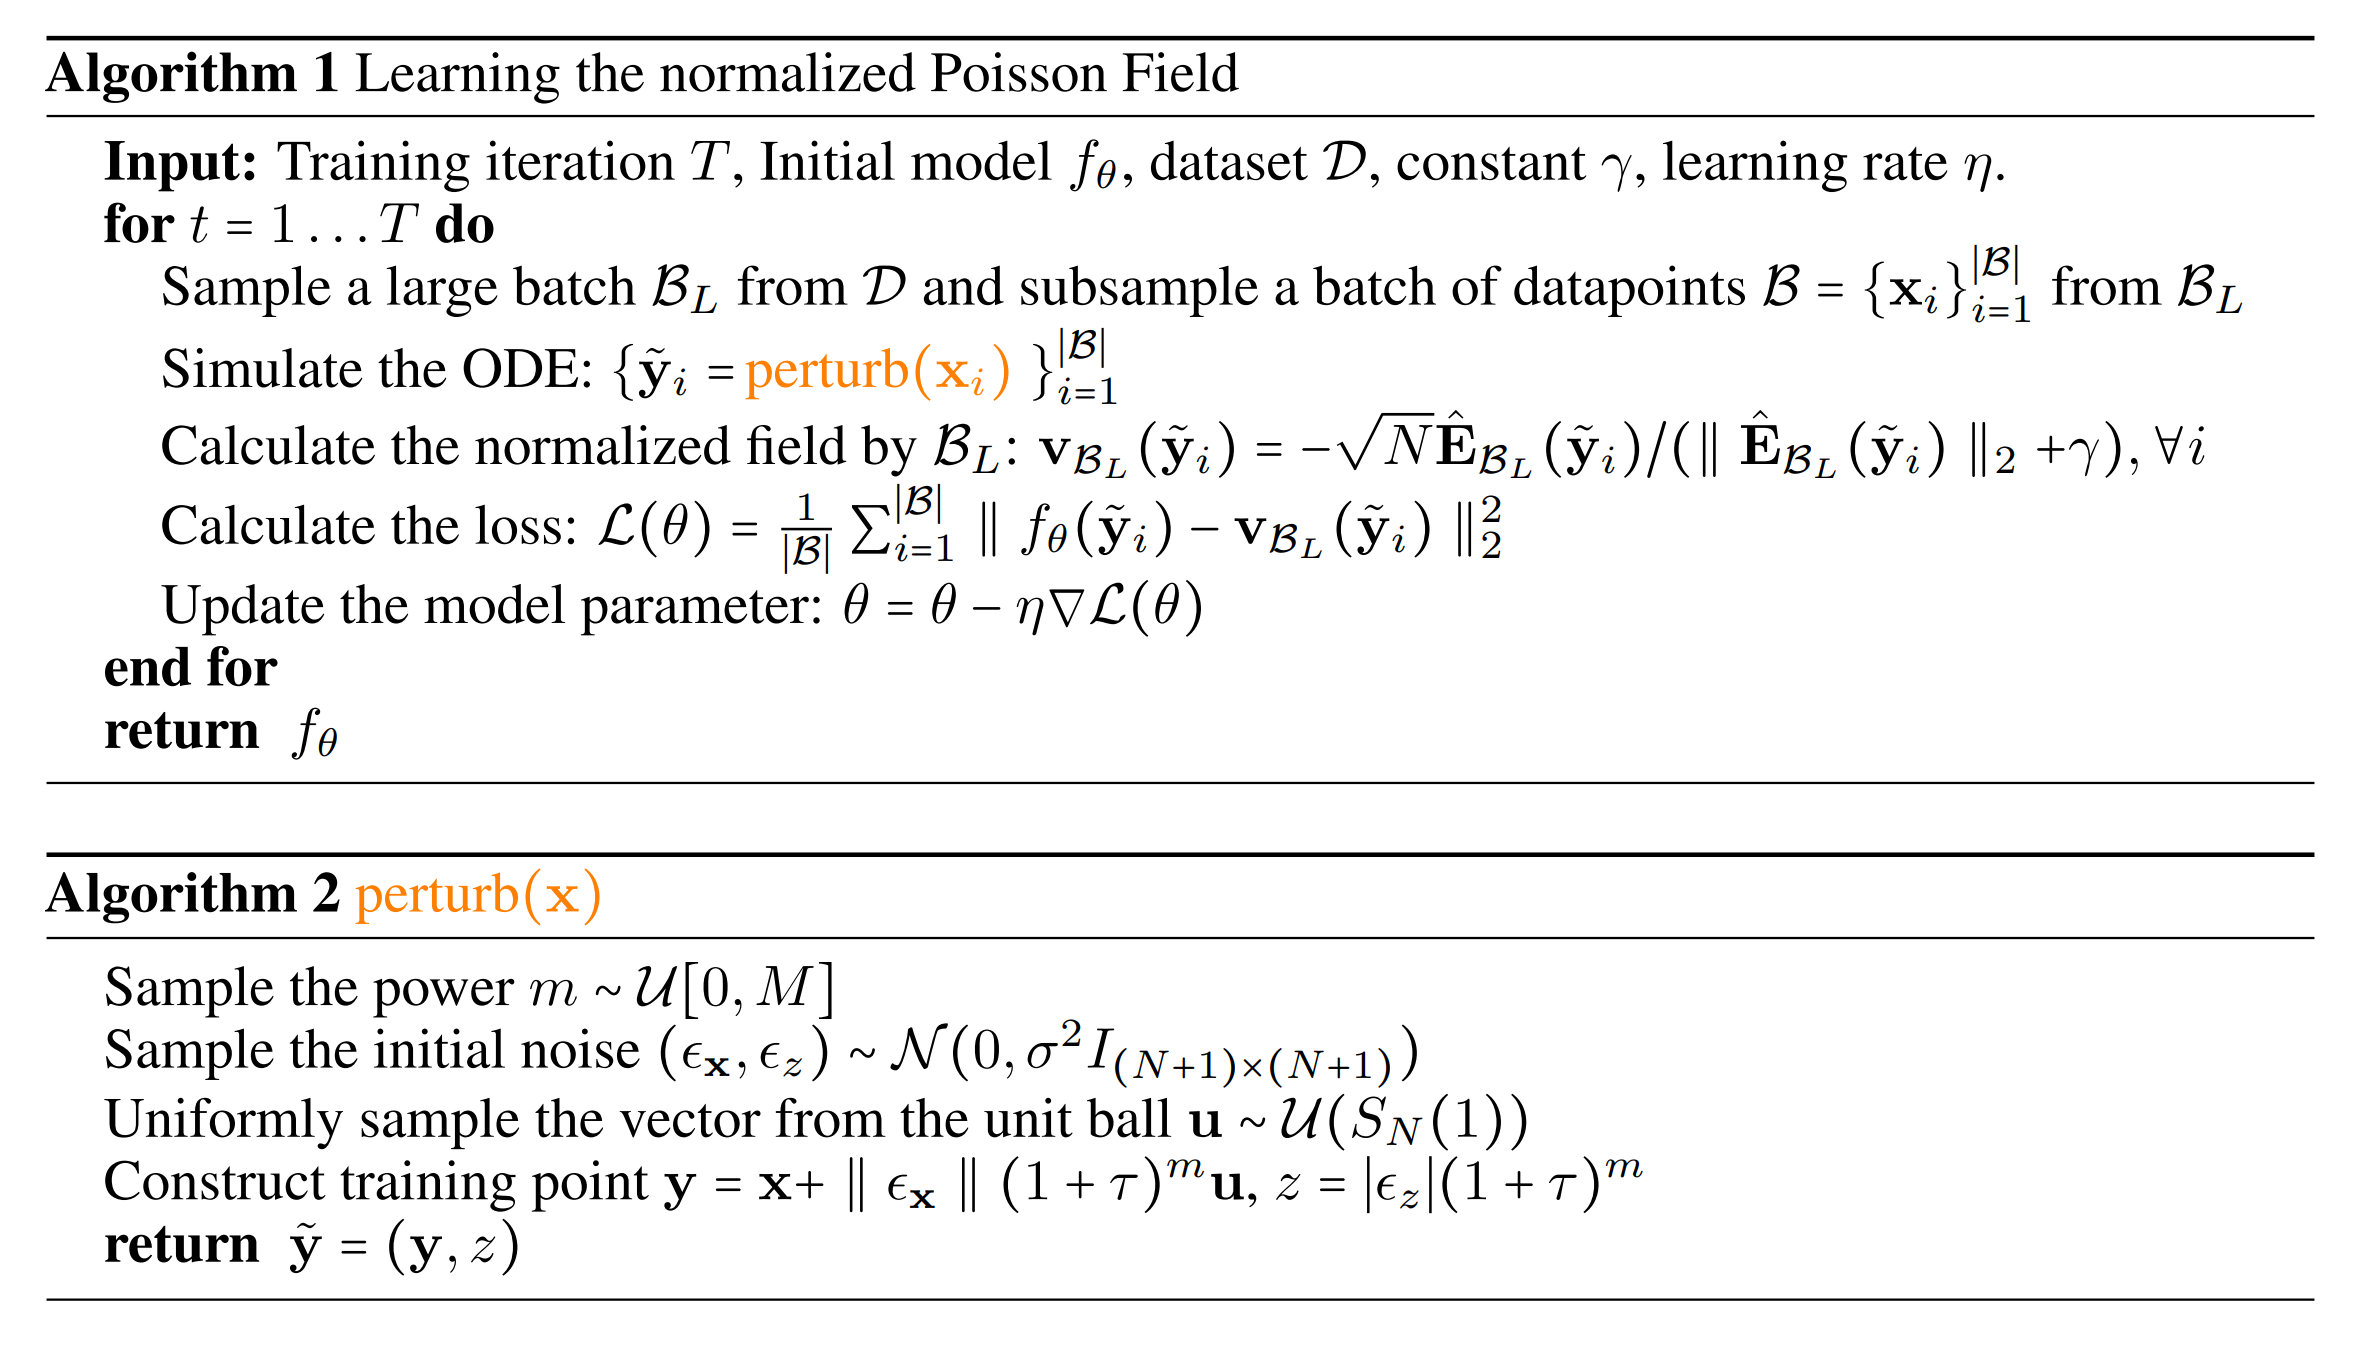
\includegraphics[width=1\textwidth]{img/algorithm.png}
\end{figure}

\subsection{附加维度锚定的后向微分方程}

在估计归一化场 $v$ 后,我们可以通过后向 ODE $d\tilde{\mathbf{x}} = v(\tilde{\mathbf{x}})dt$ 从数据分布中采样。 然而,上述 ODE 的边界条件并不明确:ODE 的起始时间和终止时间 $t$ 都是未知的。 为了解决这个问题,我们提出了一个等效的后向常微分方程,其中 $x$ 随着增广变量 $z$ 演化:
\[
  d(\mathbf{x}, z)=\left(\frac{d \mathbf{x}}{d t} \frac{d t}{d z} d z, d z\right)=\left(\mathbf{v}(\tilde{\mathbf{x}})_{\mathbf{x}} \mathbf{v}(\tilde{\mathbf{x}})_z^{-1}, 1\right) d z
\]
其中 $\mathbf{v}(\tilde{\mathbf{x}})_{\mathbf{x}}, \mathbf{v}(\tilde{\mathbf{x}})_z$ 为向量 $\mathbf{v}(\tilde{\mathbf{x}})$ 的对应 $x,z$ 分量。 在新的 ODE 中,我们将时间变量 $t$ 替换为具有物理意义的变量 $z$,从而允许显式的起始和终止条件:当 $z = 0$ 时,我们就能得到数据分布,并且可以在向后常微分方程的求解中自由选择一个较大的 $z_{\text{max}}$ 作为起始点。 后向 ODE 与通用 ODE 求解器是兼容的,例如:RK45 方法 [23] 和前向 Euler 方法。流行的简易 ODE 求解器(例如 Scipy 库 [37] 中的求解器)通常对同一批样本使用共同的起始时间。由于在 $z = z_{\text{max}}$ 超平面上的分布不再均匀,我们通过将半径为 $r = z_{\text{max}}$ 的半球上的均匀分布径向投影到 $z = z_{\text{max}}$ 超平面来导出先验分布:
\[
  p_{\text {prior }}(\mathbf{x})=\frac{2 z_{\max }^{N+1}}{S_N\left(z_{\max }\right)\left(\|\mathbf{x}\|_2^2+z_{\max }^2\right)^{\frac{N+1}{2}}}=\frac{2 z_{\max }}{S_N(1)\left(\|\mathbf{x}\|_2^2+z_{\max }^2\right)^{\frac{N+1}{2}}}
\]
其中 $S_N (r)$ 是半径为 $r$ 的 $N$ 维球体的表面积。 采用径向投影背后的原因是泊松场指向径向方向 $r \rightarrow \infty$。 新的后向 ODE 还定义了无限超平面 $(z_{\text{max}} \rightarrow \infty)$ 上的 $p_{\text{prior}}(\mathbf{x})$ 与数据分布 $\tilde{p}(\tilde{\mathbf{x}})$ 之间的双射变换,就像于定理 1 所表明的那样。从 $p_{\text{prior}}(\mathbf{x})$ 中采样的过程中,首先应当采样范数(半径):$p_{\text {radius }}\left(\|\mathbf{x}\|_2\right) \propto\|\mathbf{x}\|_2^{N-1} /\left(\|\mathbf{x}\|_2^2+z_{\max }^2\right)^{\frac{N+1}{2}}$,然后再均匀采样角度。我们在附录 A.4 中提供了详细的推导和实用的采样程序。进一步地,我们通过引入新的变量 $t'$ 实现了 $z$ 维度上的指数衰减:
\[
  \text { [Backward ODE] } \quad d(\mathbf{x}, z)=\left(\mathbf{v}(\tilde{\mathbf{x}})_{\mathbf{x}} \mathbf{v}(\tilde{\mathbf{x}})_z^{-1} z, z\right) d t^{\prime}
\]
后向 ODE 中的 $z$ 分量,即 $dz = zdt'$,可以通过 $z = e^{t'}$ 求得。 由于当 $t \rightarrow \infty$ 时 $z$ 达到零,因此我们选择一个很小的正数 $z_{\text{min}}$ 作为终止条件。 变量 $t'$ 对应的起始/终止时间分别为$\log z_{\text{max}}$/ $\log z_{\text{min}}$。 根据经验,这种简单的变量代换可以使采样速度提高 $2$ 倍,并且几乎不会损害样本质量。 此外,当 $z$ 很小时,我们用更准确的 $\mathbf{v}(\tilde{\mathbf{x}})_z$ 作为对结果的替代(附录 B.2.3)。 我们将后向 ODE 模拟的更多细节推迟到附录 B.2。

\section{通过后向微分方程进行生成建模}
本节我们将演示与 PFGM 相关的后向 ODE 在图像生成任务上的高效性。 在第 4.1 节中,我们展示了 PFGM 在 flow 模型这一系列中具有的目前最佳性能。与现有最先进的 SDE 或 MCMC 方法相比,PFGM 则表现出 $10$ 倍或 $20$ 倍的加速,兼具较高生成质量,甚至保持一定的优势。同时,与严重依赖校正器在较弱架构上生成合适样本的现有 ODE 基线不同,PFGM 表现出更高的抗错误稳定性(第 4.2 节)。 最后,我们证明 PFGM 对于欧拉方法中的步长具有鲁棒性(第 4.3 节),并且其相关 ODE 使得通过编辑增广空间实现进行似然估计和图像操作成为可能(第 4.4 节)。

\subsection{通过PFGM高效生成图像}

\textbf{设置}\quad 对于图像生成任务,我们考虑模型在 CIFAR-10 [22]、CelebA $64 \times 64$ [38] 和 LSUN bedroom  $256 \times 256$ [39]上的表现。 按照[32]提供的方法,我们首先对 CelebA 图像进行中心裁剪,然后将其大小调整为 $64 \times 64$。我们选择 $M = 291$(CIFAR-10 和 CelebA)/356(LSUN bedroom),令 $\sigma = 0.01$ 且 $\tau = 0.03$ 。而对于扰动算法 2,则在向后 ODE 中令 $z_{\text{min}} = 1e − 3$ 以及 $z_{\text{max}} = 40$ (CIFAR-10)/60 (CelebA $64^2$)/100 (LSUN bedroom)。 我们进一步将 CIFAR-10 的初始样本的范数修剪为 $(0,3000)$、CelebA $64^2$ 的初始范数修剪为 (0;6000)、LSUN bedroom 的范数修剪为 $(0,30000)$。 采用 DDPM++ 和 DDPM++ 深层架构 [33] 作为我们的框架,我们添加标量 $z$(或 $z$ 上的预测方向)作为输入(或输出)以适应附加维度。然后我们采用[33]中的同一组超参数,例如批量大小、学习率和训练迭代。附录 B.1 中提供了更多训练细节,并在 B.1.1 和 B.2.1 中讨论了如何为通用数据集设置这些超参数。

\textbf{基线}\quad 我们将 PFGM 与现代自回归模型 [36]、GAN [17, 24]、归一化流 [19] 和 EBM [8] 等模型进行比较。我们还将我们的模型与基于分数的模型的变体进行比较,例如 DDIM [30] 和当前最先进的 SDE/ODE 方法 [33]。 我们将[33]中使用前向时间 SDE 的方法表示为 Variance Exploding (VE) SDE/Variance Preserving (VP) SDE/ sub-Variance Preserving (sub-VP)。 我们还遵循[33]中的模型选择指导,认为在每 $50k$ 次迭代的训练过程中应当选择具有最小 FID 分数的检查点。

\textbf{数值求解器}\quad 后向 ODE(方程(6))与任何通用 ODE 求解器都是兼容的。 在我们的实验中,除非另有说明,ODE 的默认求解器是 Scipy 库 [37] 中使用 RK45 [7] 方法 (RK45) 的求解器。 对于 VE/VP/subVP-SDE,我们使用[33]中介绍的预测-校正(PC)采样器。 对于 VP/sub-VP-SDE,我们应用仅预测采样器,因为它的性能与 PC 采样器相当,但仅需要一半的计算量。

\begin{figure}[ht]
  \centering
  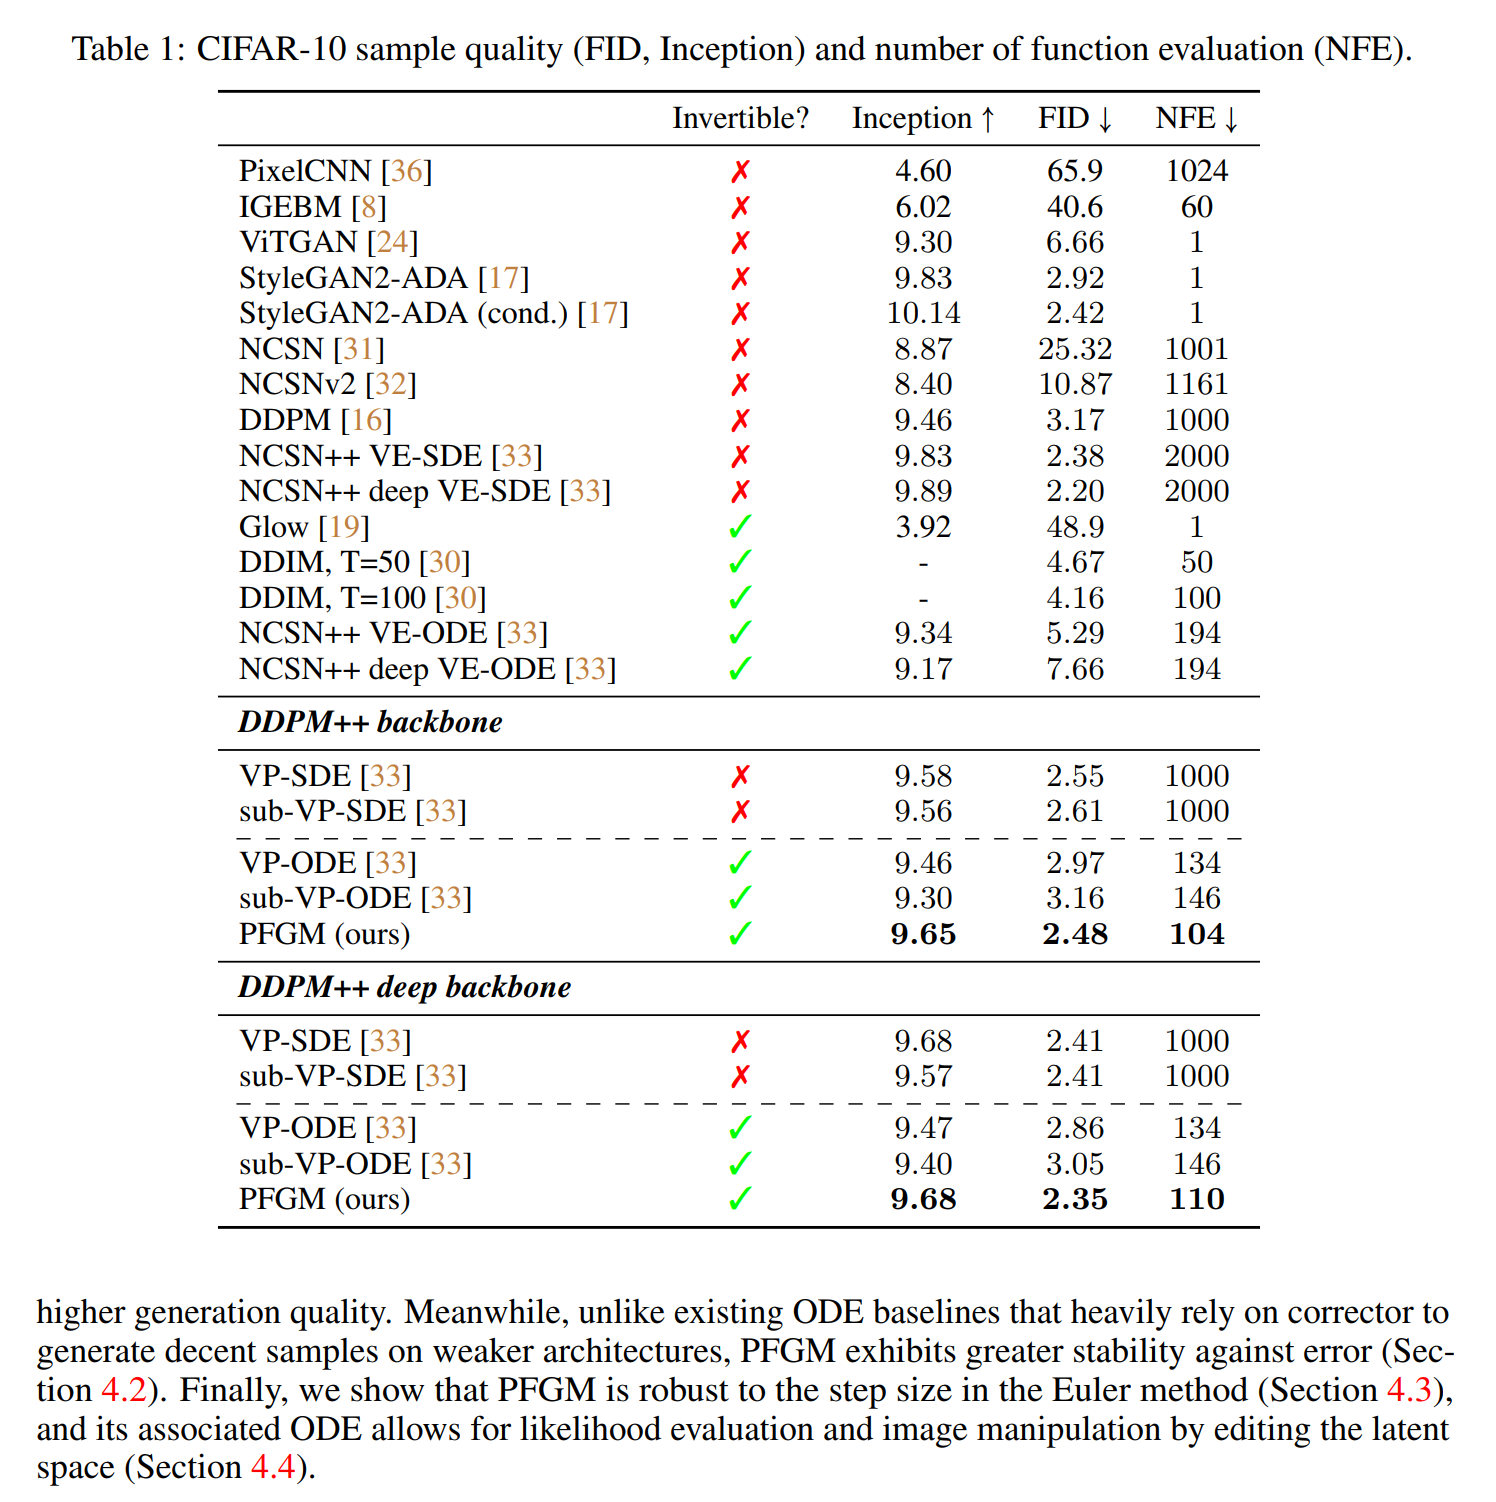
\includegraphics[width=1\textwidth]{img/table1.png}
\end{figure}

\textbf{结果}\quad 对于 CIFAR-10 的定量评估,我们在表 $1$ 中报告了 Inception [29](越高越好)以及 FID [13] 的分数(越低越好)。另外还包括了我们在较弱架构 NCSNv2 上的初步实验结果 [32] ,见附录 D.2。 通过平均 NFE(函数评估次数)来衡量推理速度,我们还明确指出哪些方法属于可逆流模型这一系列。

我们的主要发现是:\textbf{(1)PFGM 在归一化流模型中实现了最佳的 Inception 分数和 FID 分数。} 具体来说,PFGM 使用 DDPM++ 深度架构获得了 $9.68$ 的 Inception 分数和 $2.48$ 的 FID 分数。 据我们所知,这些是 CIFAR-10 数据集上流模型的最高 FID 和 Inception 分数。 \textbf{(2) PFGM 比使用类似架构的 SDE 方法实现了 $10\backsim 20$ 的推理速度,同时保持了相当的样本质量。} 如表 $1$ 所示,PFGM 需要 $110$ 个 NFE,而 SDE 方法通常使用 $1000$ 至 $2000$ 个推理步骤,并且 PFGM 在所有指标中均优于 DDPM++ 的所有基线。 此外,使用相同的 RK45 求解器,PFGM 的采样速度通常也比其他 ODE 基线更快。 \textbf{(3) PFGM 中的后向 ODE 与不同容量的框架结构兼容。} PFGM 在 DDPM++(表 $1$)或 NCSNv2(附录 D.2)的主干数据上始终优于其他 ODE 基线。 \textbf{(4) PFGM 显示出对更高分辨率数据集的可扩展性。} 在附录 D.1 中,我们表明 PFGM 能够扩展到 LSUN bedroom $256\times 256$ 数据集。另外值得注意的是 PFGM 的性能与 VE-SDE 相当,但 NFE 减少了 $15$ 倍。

\begin{figure}[ht]
  \centering
  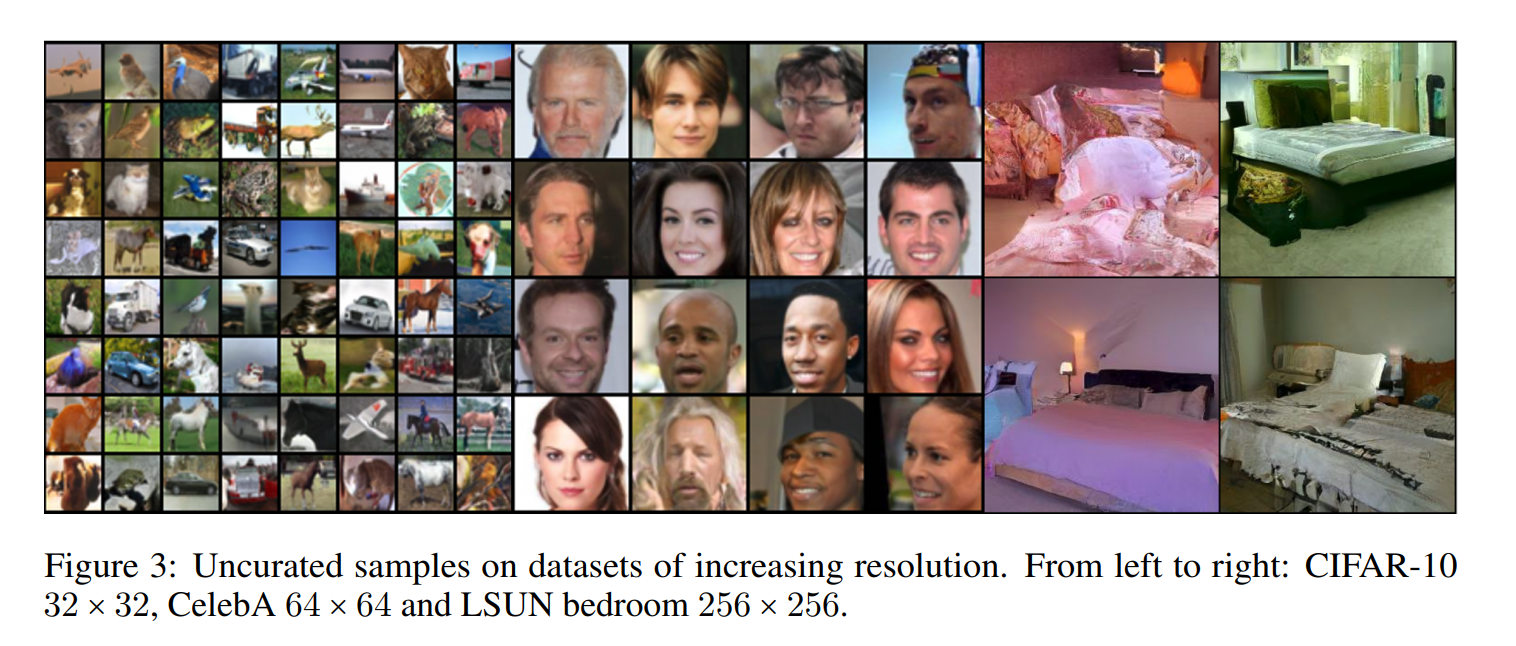
\includegraphics[width=1\textwidth]{img/figure3.png}
\end{figure}

在图 $3$ 中,我们在 CIFAR-10、CelebA $64 \times 64$ 数据集和 LSUN bedroom $256 \times 256$ 数据集上可视化来自 PFGM 的未整理样本。附录 E 则提供了更多样本。

\subsection{ VE/VP-ODE 模型在 NCSNv2 架构上的问题}

在我们对 NCSNv2 框架的初步实验中,我们凭经验观察到 VE/VP-ODE 在 CIFAR-10 数据集上的 FID 分数大于 $90$。 特别是,VE/VP-ODE 仅在应用 Langevin 动力学校正器时才能生成不错的样本,即使如此,它们的性能仍然不如 PFGM(表 9、表 10)。这一模型在 NCSNv2 上的较差性能与[33]中 NCSN++/DDPM++ 上的高样本质量形成鲜明对比。\textbf{这表明 VE/VP-ODE 比 PFGM 更容易受到估计误差的影响。}我们假设在基于分数的模型训练期间出现的强范数-$\sigma$ 相关性导致了这一问题。

\begin{figure}[ht]
  \centering
  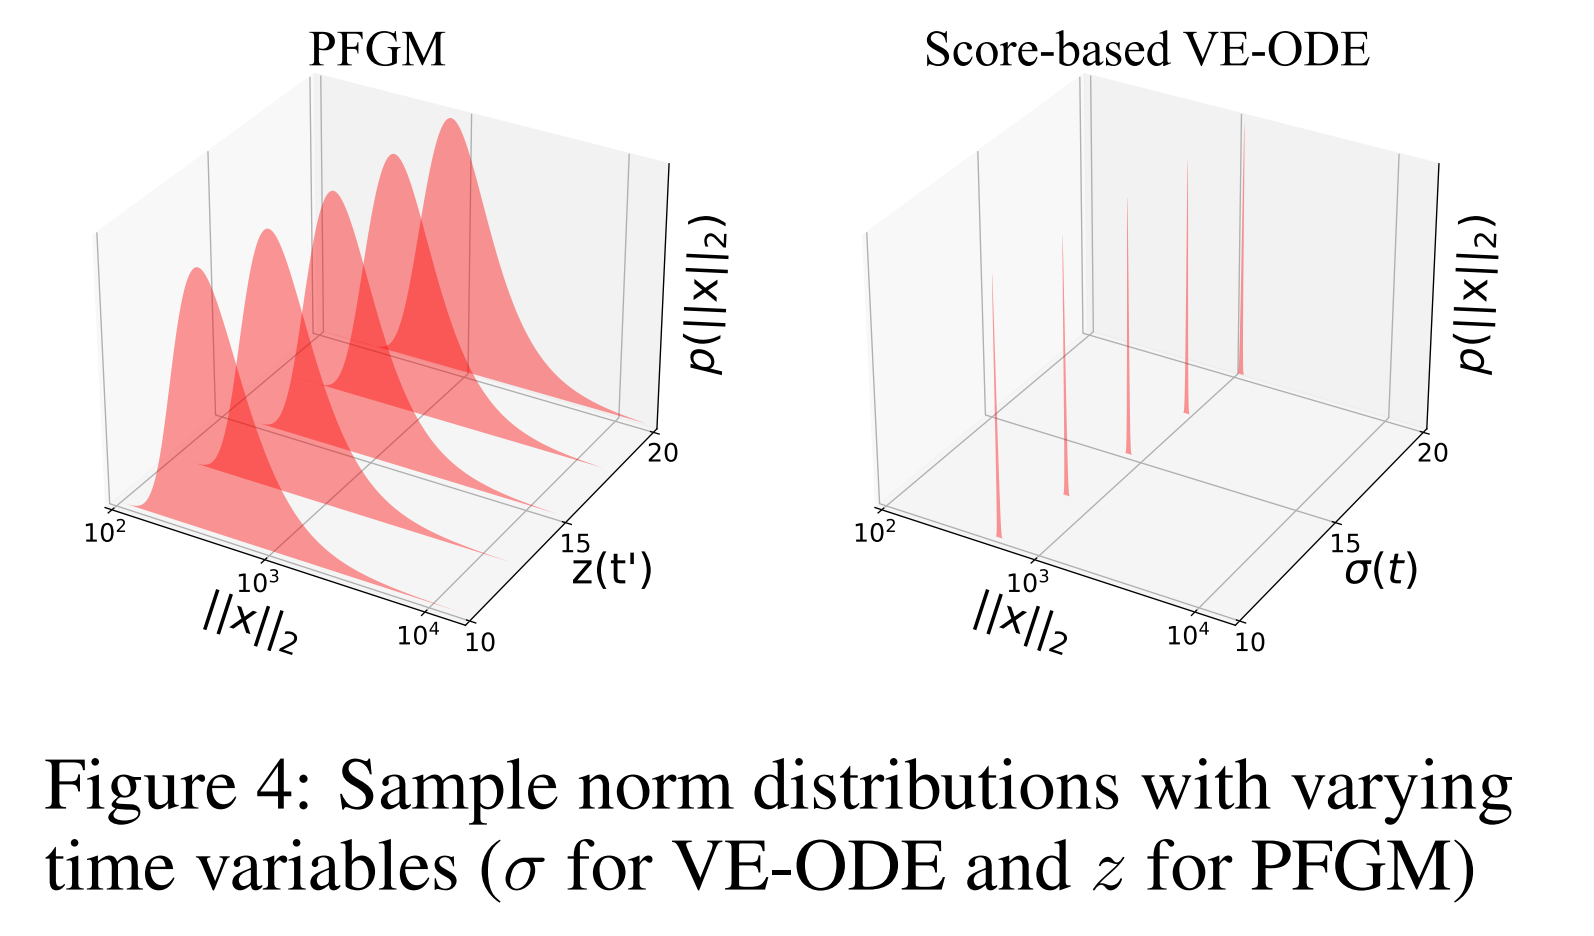
\includegraphics[width=0.5\textwidth]{img/figure4.png}
\end{figure}

对于基于分数的模型,扰动训练样本的 $l_2$ 范数和高斯噪声的标准差 $\sigma(t)$ 具有很强的相关性,例如:对于 VE 中的大 $\sigma(t)$,$l_2$ 范数约为 $\sigma(t)\sqrt{N}$ [33]。 相比之下,如图 4 所示,PFGM 在广泛的训练样本范数中都有着较高的生成质量。在采样过程中,当后向 ODE 的轨迹偏离大多数训练样本所属的范数 $\sigma(t)$ 关系时,VE/VP-ODE 可能会崩溃。较弱的 NCSNv2 主干网会产生较大的错误,从而导致其失败。但是由于训练样本范数范围更大,PFGM 更能抵抗估计上的错误。

\begin{figure}[ht]
  \centering
  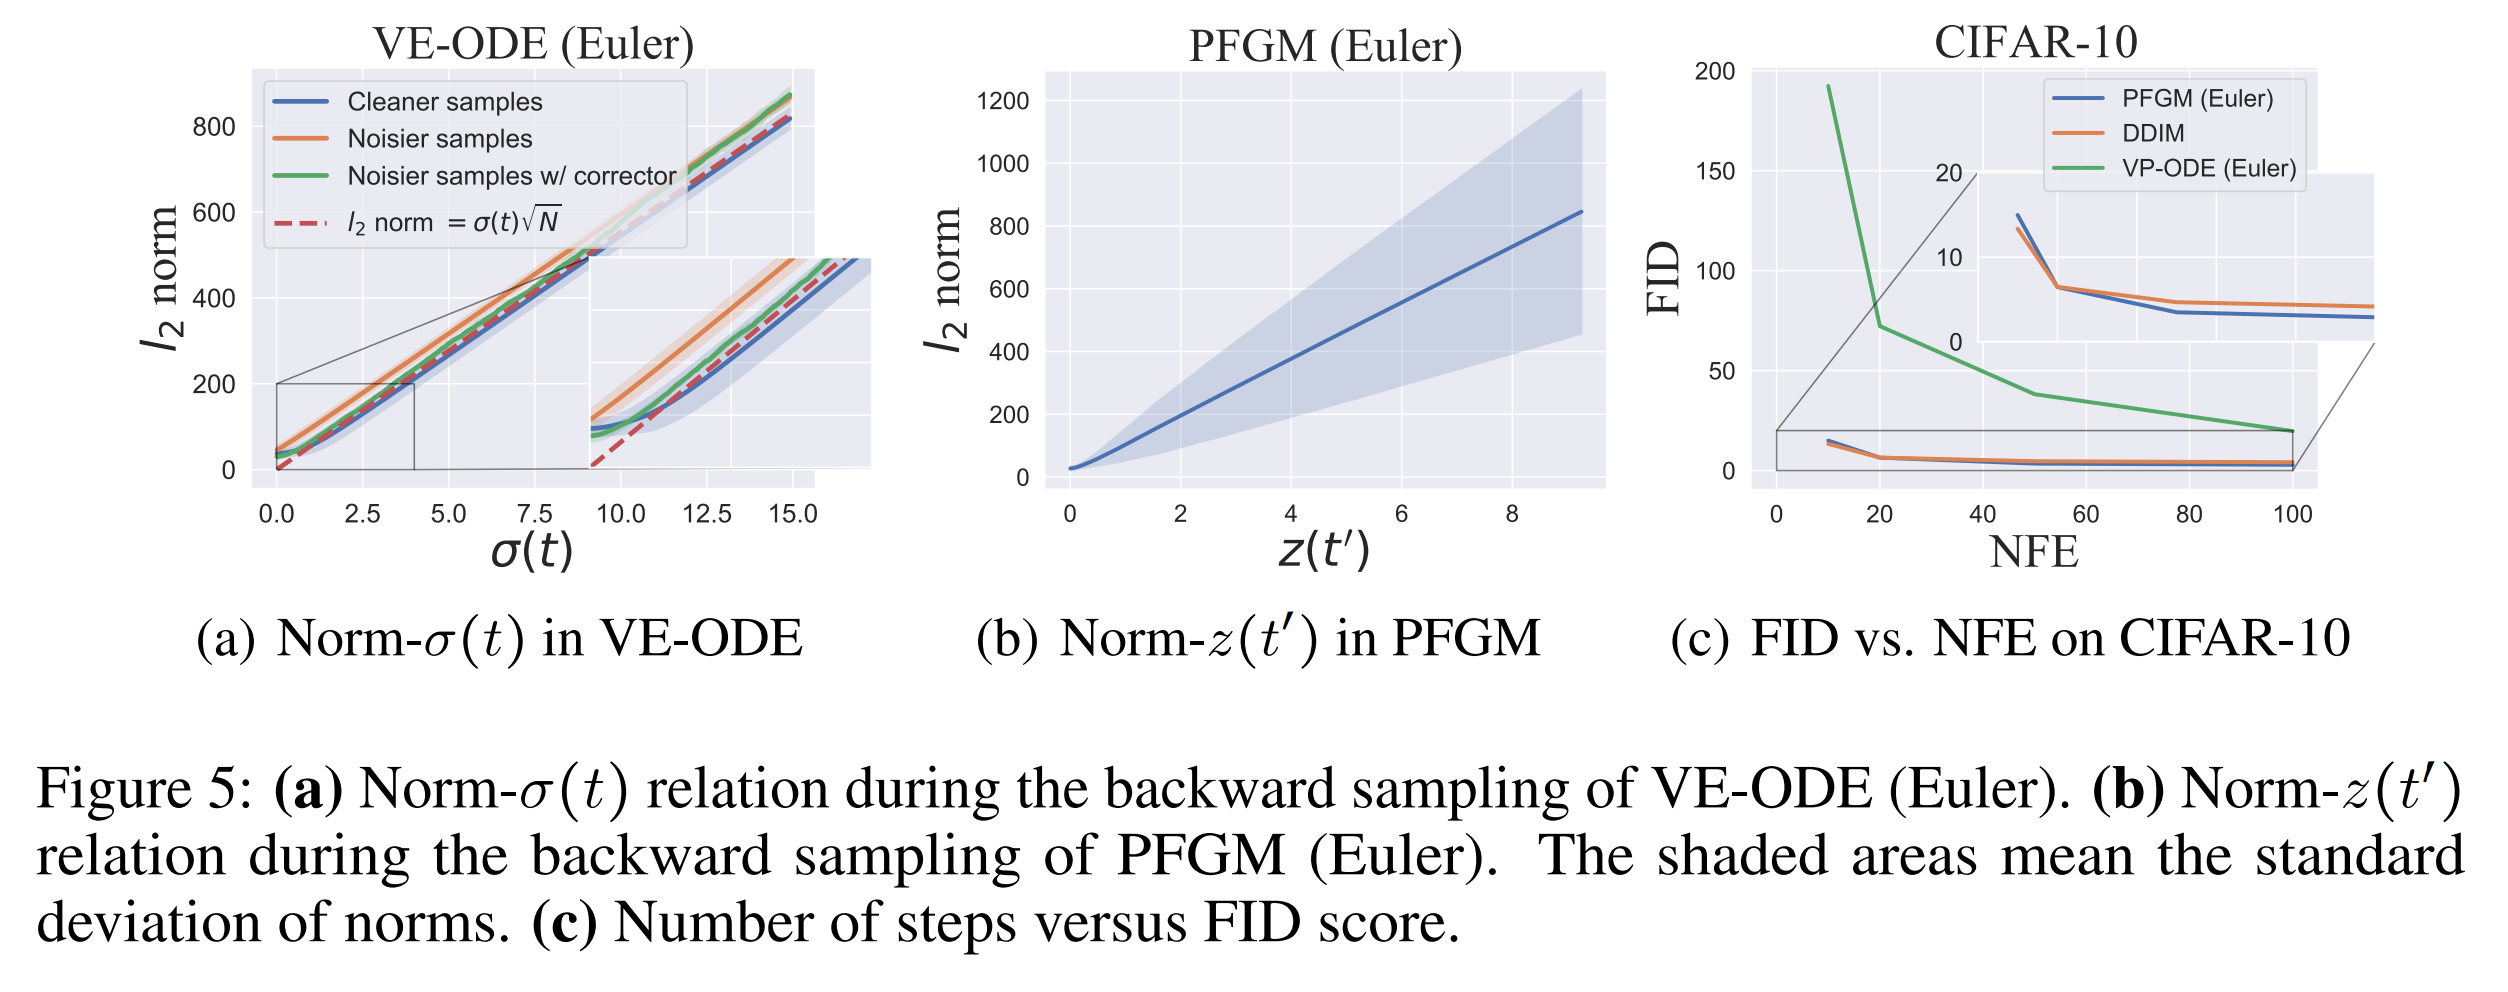
\includegraphics[width=1\textwidth]{img/figure5.png}
\end{figure}

为了进一步验证上述假设,我们根据图片质量将一批 VE-ODE 样本分为更干净的样本和更嘈杂的样本(图8(a))。 在图 5(a)中,我们研究了当 $\sigma(t) < 15 $时,在 VE-ODE 的前向欧拉模拟过程中,干净样本和噪声样本的关系。可以看到,干净样本的轨迹接近范数-$\sigma (t)$ 关系(红色虚线),而噪声较大的样本的关系偏离该关系。 Langevin 动力学校正器可以改变噪声样本的轨迹以与关系保持一致。 图5(b)进一步表明,锚定变量$z(t')$与 PFGM 后向 ODE 中的范数不存在任何的强相关,从而对于在 NCSNv2 上的不精确估计具有鲁棒性。 我们将更多细节放在附录 C 中讨论。

\subsection{前向欧拉方法中步长的影响}

为了加快 ODE 的求解速度,我们可以增加数值求解器(例如前向欧拉法)的步长(减小 NFE)。 它还可以在实际部署中实现样本质量和计算效率之间的权衡。 我们使用前向欧拉方法研究增加步长对 PFGM、VP-ODE 和 DDIM [30] 的影响,NFE 范围是从 $10$ 到 $100$。

在图 5(c) 中,我们报告了通过 CIFAR-10 上的 FID 评分衡量的样本质量。 正如预期的那样,当降低 NFE 时,所有的方法都具有更高的 FID 分数。 但当 NFE 降低时,PFGM 的样本质量会适度下降。 我们的方法对步长的鲁棒性明显优于 VP-ODE,尤其是在仅采用几个欧拉步时。 此外,在大多数 NFE 上,PFGM 获得比 DDIM 更好的 FID 分数,但 $10$ 个 NFE 分数的除外,并且 PFGM 稍差。 这表明 PFGM 是一种适应瞬时资源可用性的有前途的方法,因为可以在有限的步骤中生成高质量的样本。

\subsection{似然估计与潜在表示}

与离散归一化流模型[6,19,14]和连续概率流模型[33]类似,PFGM 中的前向 ODE 定义了数据空间和具有已知先验的潜在空间之间的可逆映射。 形式上,我们通过积分方程对应的前向 ODE $d(\mathbf{x}, z)=\left(\mathbf{v}(\tilde{\mathbf{x}})_{\mathbf{x}} \mathbf{v}(\tilde{\mathbf{x}})_z^{-1} z, z\right) d t^{\prime}$ 来定义可逆前向 $\mathcal{M}$ 映射:
\[
  \mathbf{x}\left(\log z_{\max }\right)=\mathcal{M}\left(\mathbf{x}\left(\log z_{\min }\right)\right) \equiv \mathbf{x}\left(\log z_{\min }\right)+\int_{\log z_{\min }}^{\log z_{\max }} \mathbf{v}\left(\mathbf{x}\left(t^{\prime}\right)\right)_{\mathbf{x}} \mathbf{v}\left(\tilde{\mathbf{x}}\left(t^{\prime}\right)\right)_z^{-1} e^{t^{\prime}} d t^{\prime}
\]
其中 $\log z_{\min} / \log z_{\max}$ 是正向 ODE 中的起始/终止时间。 正向映射将数据分布映射到 $z = z_{\max}$ 超平面上的先验分布 $p_\text{prior}$(参见第 3.3 节):$p_{\text {prior}}\left(\mathbf{x}\left(\log z_{\max}\right)\right)=\mathcal{M}\left(p\left(\mathbf{x}\left(\log z_{\min}\right)\right)\right)$,而映射的可逆性使得我们可以对它进行似然估计,并在 $z = z_{\max}$ 的超平面上创建有意义的潜在空间。 此外,我们还可以通过调整数值 ODE 求解器的步长或精度来适应计算机的相应约束。

\textbf{似然估计}\quad 我们通过变量的瞬时变化公式[4, 33]对数据进行似然估计。 在表 2 中,我们报告了统一去量化的 CIFAR-10 测试集上的 bits/dim 值,并与使用相同设置的现有基线进行了比较。 我们观察到,即使没有极大似然的训练,PFGM 也能比离散归一化流模型获得更好的似然结果。 在连续流模型中,sub-VP-ODE 显示了最低的 bits/dim 值,尽管其样本质量比 VP-ODE 和 PFGM 差(表 1)。对与似然程度与样本质量之间可能的权衡,则留给后来者去探索。

\begin{figure}[ht]
  \centering
  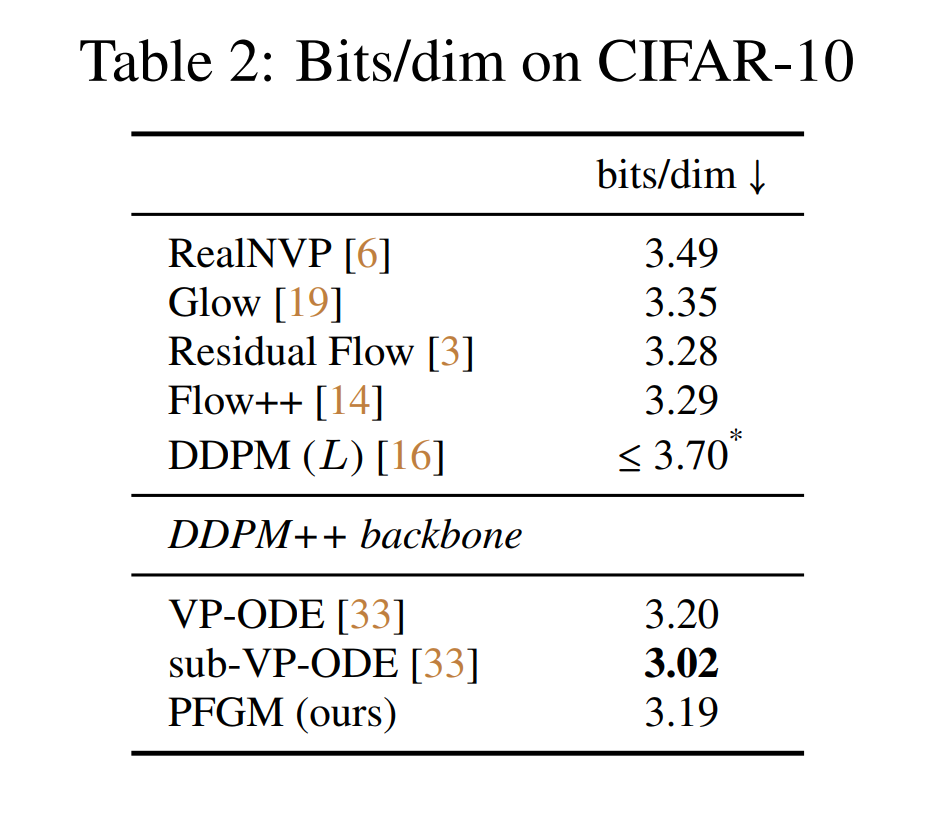
\includegraphics[width=0.5\textwidth]{img/table2.png}
\end{figure}

\textbf{潜在表示}\quad 由于样本可以通过可逆映射 $\mathcal M$ 来唯一确定,因此 PFGM 使用其在 $z = z_{\max}$ 超平面上的潜在表示来进一步支持图像操作。 我们将图像插值和温度缩放的结果[6,19,33]分别放在附录 D.4 和附录 D.5 中。而对于数据的插值,它表明我们可以沿着潜在空间行进以获得在 CelebA 图像之间在感官上一致的插值。

\section{总结}

本文通过求解场源是数据分布的泊松方程提出了一种新的深度生成模型,并在具有附加维度的增广空间中求解归一化梯度场。在采样过程中我们设计了一个后向 ODE ,它的解在有物理意义的附加维度上呈指数衰减。在实验上,我们的方法目前比其他归一化流模型具有更优良的性能,并且相对随机方法实现了 $10$ 倍至 $20$ 倍的加速。 与流行的基于 ODE 的方法相比,我们的后向 ODE 显示出更高的抗误差稳定性,并且能够实现高效的自适应采样。此外,我们进一步证明了前向 ODE 在似然评估和图像插值方面的实用性。本工作未来的发展方向包括对泊松场标准化过程的改进,可以使用更具有一定规则的方法来解决不同的近场行为。例如,我们可以利用重整化(物理学中的一个有用工具)来优化泊松场在近场中的表现。

\bibliography{ustc}  % 参考文献使用 BibTeX 编译
% \printbibliography       % 参考文献使用 BibLaTeX 编译

\[
  d\mathbf{x} = \mathbf{f}(\mathbf{x},t)dt + g(t)d\mathbf{w}
\]

\end{document}